\documentclass[12pt]{article}
\usepackage[usenames]{color} %used for font color
\usepackage{amsmath,amssymb,amsthm,amsfonts} %maths
\usepackage[utf8]{inputenc} %useful to type directly accentuated characters
\usepackage{hyperref}
\usepackage[top=1in, bottom = 1in, left = 0.75in, right = 0.75in]{geometry}
\usepackage{graphicx}
\usepackage{tcolorbox}
\usepackage{listings}
\usepackage{booktabs}

\definecolor{codegreen}{rgb}{0,0.6,0}
\definecolor{codegray}{rgb}{0.5,0.5,0.5}
\definecolor{codepurple}{rgb}{0.58,0,0.82}
\definecolor{backcolour}{rgb}{0.95,0.95,0.92}

\lstdefinestyle{mystyle}{
    backgroundcolor=\color{backcolour},   
    commentstyle=\color{codegreen},
    keywordstyle=\color{magenta},
    numberstyle=\tiny\color{codegray},
    stringstyle=\color{codepurple},
    basicstyle=\ttfamily\footnotesize,
    breakatwhitespace=false,         
    breaklines=true,                 
    captionpos=b,                    
    keepspaces=true,                 
    numbers=left,                    
    numbersep=5pt,                  
    showspaces=false,                
    showstringspaces=false,
    showtabs=false,                  
    tabsize=2
}

\lstset{style=mystyle}

\setlength\parindent{0pt}


\newtheoremstyle{problemstyle}  							% <name>
        {3pt}                                               % <space above>
        {3pt}                                               % <space below>
        {\normalfont}                               		% <body font>
        {}                                                  % <indent amount}
        {\bfseries}                 						% <theorem head font>
        {\normalfont\bfseries.}         					% <punctuation after theorem head>
        {.5em}                                          	% <space after theorem head>
        {}                                                  % <theorem head spec (can be left empty, meaning `normal')>
\theoremstyle{problemstyle}

\newtheorem{pbm}{Problem}
\newtheorem{solution}{Solution}
\newtheorem*{solution*}{Solution}

\newenvironment{problem}{
\begin{tcolorbox}[colback=green!10!white,colframe=black!75!black, parbox = false]\begin{pbm} }{\end{pbm}\end{tcolorbox} }


\makeatletter
\newcommand*\bigcdot{\mathpalette\bigcdot@{.5}}
\newcommand*\bigcdot@[2]{\mathbin{\vcenter{\hbox{\scalebox{#2}{$\m@th#1\bullet$}}}}}
\makeatother


\newcommand{\prob}{\mathbb{P}}
\newcommand{\E}{\mathbb{E}}
\newcommand{\Var}{\mathbb{V}}
\newcommand{\normal}{\mathcal{N}}
\newcommand{\Sample}{\mathcal{S}}
\newcommand{\R}{\mathbb{R}}
\newcommand{\C}{\mathbb{C}}
\newcommand{\N}{\mathbb{N}}
\newcommand{\Q}{\mathbb{Q}}
\newcommand{\Z}{\mathbb{Z}}
\newcommand{\indep}{\mathrel{\text{\scalebox{1.07}{$\perp\mkern-10mu\perp$}}}}
\newcommand{\ind}[1]{\mathbf{1}_{ \{#1\} }}
\newcommand{\bb}[1]{\boldsymbol{#1}}
\newcommand{\transpose}{^\intercal}


\begin{document}

\begin{titlepage}
    \begin{center}
        \vspace*{3cm}
        \Huge{\textbf{Statistical Inference 2 Assignment 2}}\\
        \vspace*{1cm}
        \large{\textit{Master of Statistics (M.Stat.) Year II, Session 2020-21}}\\
        \vspace*{5cm}
        \begin{tcolorbox}[colback=black!5!white,colframe=black!75!black, width = 0.5\linewidth]
            \vspace*{0.5cm}
            \textbf{Name: } Subhrajyoty Roy\\
            \textbf{Roll: } MB1911
            \vspace*{0.5cm}
        \end{tcolorbox}
    \end{center}
    \vspace*{3cm}
    \begin{flushright}
        \large\textit{\today}
    \end{flushright}
\end{titlepage}

\begin{problem}
    Consider the linear regression model $\bb{y} = \bb{X}\bb{\beta} + \bb{\epsilon}$ where $\bb{y} = (y_1, \dots y_n)'$ is the vector of observations on the ``dependent'' variable, $\bb{X} = ((x_{ij}))_{n\times p}$ is of full rank, $x_{ij}$ being the values of the nonstochastic regressor variables, $\bb{\beta} = (\beta_1, \dots \beta_p)'$ is the vector of regression coefficients and the components of $\bb{\epsilon}$ are independent, each following $\normal(0, \sigma^2)$. Consider the noninformative prior $\pi(\beta, \sigma^2) \propto \sigma^{-2}, \bb{\beta} \in \R^p, \sigma^2 > 0$.
    \begin{enumerate}
        \item[(a)] Find the $100(1-\alpha)\%$ HPD credible set for $\bb{\beta}$.
        \item[(b)] Find the marginal posterior distribution of a particular $\beta_j$ ($j = 1, \dots p$) and use it to find the $100(1 -\alpha)\%$ HPD credible set for $\beta_{j}$. 
    \end{enumerate}
\end{problem}

\begin{solution*}
    \begin{enumerate}
        \item[(a)] Since, $\bb{y} = \bb{X}\bb{\beta} + \bb{\epsilon}$ and each component of $\bb{\epsilon}$ are independent, following $\normal(0, \sigma^2)$, clearly $\bb{y}$ has a $n$-variate multivariate normal distribution with mean parameter $\bb{X}\bb{\beta}$ and dispersion matrix $\sigma^2 \bb{I}_n$, where $\bb{I}_n$ is the identity matrix of order $n$.
        
        We start by writing the joint posterior of $(\bb{\beta}, \sigma^2)$ as,
        
        \begin{align*}
            \pi(\bb{\beta}, \sigma^2 \mid \bb{X}, \bb{y}) 
            & \propto \pi(\bb{\beta}, \sigma^2) \mathcal{L}(\bb{y}\mid \bb{X}, \bb{\beta}, \sigma^2), \qquad \text{since, } \bb{X} \text{ is nonstochastic}\\
            & \propto \dfrac{1}{\sigma^2} \times \dfrac{1}{\det(\sigma^2 \bb{I}_n)^{1/2}} e^{-\frac{1}{2\sigma^2} (\bb{y} - \bb{X}\bb{\beta})\transpose (\bb{y} - \bb{X}\bb{\beta})} \\
            & = \sigma^{-(n+2)} \exp\left[ -\dfrac{1}{2\sigma^2} (\bb{y} - \bb{X}\bb{\beta})\transpose (\bb{y} - \bb{X}\bb{\beta}) \right]
        \end{align*}

        Denoting $\widehat{\bb{\beta}}$ as the ordinary least square regression estimate of $\bb{\beta}$, the quantity $(\bb{y} - \bb{X}\bb{\beta})\transpose (\bb{y} - \bb{X}\bb{\beta})$ can be decomposed as,

        \begin{align*}
            (\bb{y} - \bb{X}\bb{\beta})\transpose (\bb{y} - \bb{X}\bb{\beta})
            & = (\bb{y} - \bb{X}\widehat{\bb{\beta}} + \bb{X}(\widehat{\bb{\beta}} - \bb{\beta}) )\transpose (\bb{y} - \bb{X}\widehat{\bb{\beta}} + \bb{X}(\widehat{\bb{\beta}} - \bb{\beta}))\\
            & = (\bb{y} - \widehat{\bb{y}})\transpose (\bb{y} - \widehat{\bb{y}}) + 2(\bb{y} - \widehat{\bb{y}})\transpose \bb{X} (\widehat{\bb{\beta}} - \bb{\beta}) + (\bb{\beta} - \widehat{\bb{\beta}})\transpose \bb{X}\transpose \bb{X} (\bb{\beta} - \widehat{\bb{\beta}})\\
            & \qquad \qquad \qquad \text{ where, } \widehat{\bb{y}} = \bb{X}\widehat{\bb{\beta}}\\
            & = (\bb{y} - \widehat{\bb{y}})\transpose (\bb{y} - \widehat{\bb{y}}) + (\bb{\beta} - \widehat{\bb{\beta}})\transpose \bb{X}\transpose \bb{X} (\bb{\beta} - \widehat{\bb{\beta}})
        \end{align*}

        since, the residual $(\bb{y} - \widehat{\bb{y}})$ belongs to the orthogonal complement of the column space of $\bb{X}$. Denoting the first term $SSE = (\bb{y} - \widehat{\bb{y}})\transpose (\bb{y} - \widehat{\bb{y}})$, we have 

        $$
        \pi(\bb{\beta}, \sigma^2 \mid \bb{X}, \bb{y}) \propto \sigma^{-(n+2)} \exp\left[ -\dfrac{1}{2\sigma^2}  (SSE + (\bb{\beta} - \widehat{\bb{\beta}})\transpose \bb{X}\transpose \bb{X} (\bb{\beta} - \widehat{\bb{\beta}}))  \right]
        $$

        Therefore, the posterior distribution of $\bb{\beta}$ can be obtained as,

        \begin{align*}
            \pi(\bb{\beta}, \mid \bb{X}, \bb{y})
            & = \int_0^\infty \pi(\bb{\beta}, \sigma^2 \mid \bb{X}, \bb{y}) d(\sigma^2)\\
            & \propto \int_0^\infty \sigma^{-(n+2)} \exp\left[ -\dfrac{1}{2\sigma^2} (SSE + (\bb{\beta} - \widehat{\bb{\beta}})\transpose \bb{X}\transpose \bb{X} (\bb{\beta} - \widehat{\bb{\beta}}))  \right] d(\sigma^2)\\
            & \propto \left[ SSE + (\bb{\beta} - \widehat{\bb{\beta}})\transpose \bb{X}\transpose \bb{X} (\bb{\beta} - \widehat{\bb{\beta}}) \right]^{-n/2}\\
            & \propto \left[ 1 + \dfrac{(\bb{\beta} - \widehat{\bb{\beta}})\transpose \bb{X}\transpose \bb{X} (\bb{\beta} - \widehat{\bb{\beta}})}{SSE} \right]^{-n/2}\\
            & = \left[ 1 + \dfrac{(\bb{\beta} - \widehat{\bb{\beta}})\transpose \bb{X}\transpose \bb{X} (\bb{\beta} - \widehat{\bb{\beta}})}{(n-p)s^2} \right]^{-((n-p)+p)/2}, \ \text{where } s^2 = \dfrac{(\bb{y} - \widehat{\bb{y}})\transpose (\bb{y} - \widehat{\bb{y}})}{(n-p)}
        \end{align*}

        Denoting $\Sigma_X = \bb{X}\transpose \bb{X}$, we have the posterior distribution of $\bb{\beta}$ is a multivariate $t$ distribution with $(n-p)$ d.f. ($p$ is the number of predictors), location parameter $\widehat{\bb{\beta}}$ (the OLS estimate of $\bb{\beta}$) and the scale or dispersion parameter $\Sigma_X^{-1/2}s$. In other words, the quantity

        $$
        F(\bb{\beta}) = \dfrac{\dfrac{(\bb{\beta} - \widehat{\bb{\beta}})\transpose \bb{X}\transpose \bb{X} (\bb{\beta} - \widehat{\bb{\beta}})}{p}}{\dfrac{(n-p)s^2}{(n-p)}} = \dfrac{(\bb{\beta} - \widehat{\bb{\beta}})\transpose \bb{X}\transpose \bb{X} (\bb{\beta} - \widehat{\bb{\beta}})}{ps^2}
        $$

        \noindent has a $F_{p, (n-p)}$ distribution. Therefore, an obvious $100(1-\alpha)\%$ HPD credible set can be given based on the ellipsoid 

        $$
        \left\{ \bb{\beta} : F(\bb{\beta}) \leq F_{p, n-p, \alpha} \right\} = \left\{ \bb{\beta} : (\bb{\beta} - \widehat{\bb{\beta}})\transpose \bb{X}\transpose \bb{X} (\bb{\beta} - \widehat{\bb{\beta}}) \leq ps^2 F_{p, n-p, \alpha} \right\}
        $$

        \noindent where $F_{p, n-p,\alpha}$ is the $(1-\alpha)$-th quantile of the $F_{p, n-p}$ distribution. (The HPD property follows from the unimodality and symmetricity of the multivariate $t$ distribution).

        \item[(b)] For this, we shall use the following result that if $\bb{x}_{n \times 1}$ is a random variable following a multivariate $t$ distribution of $r$ d.f. with location parameter $\mu$ and dispersion matrix $\Sigma$, then a linear combination of its components, i.e. for any nonstochastic vector $\bb{a}_{n \times 1}$, the random variable $y = \bb{a}\transpose \bb{x}$ has a univariate $t$ distribution of $r$ d.f., with location parameter $\bb{a}\transpose \mu$ and scale parameter $\bb{a}\transpose \Sigma \bb{a}$.
        
        For $j = 1, 2, \dots p$, let, $\bb{e}_j$ be the column vector of size $p$ such that only its $j$-th coordinate is equal to $1$ and all other coordinates are equal to $0$. Using this result for the posterior distribution of $\bb{\beta}$, we obtain $\beta_j = \bb{e}_j\transpose \bb{\beta}$, has the posterior distribution as a univariate $t$ distribution with $(n-p)$ d.f., but with the location parameter $\bb{e}_j\transpose \widehat{\bb{\beta}} = \widehat{\beta}_j$ (which is the $j$-th coordinate of the OLS estimate $\widehat{\bb{\beta}}$), and the scale parameter, 
        
        $$
        \bb{e}_j\transpose (\Sigma_X^{-1/2} s) \bb{e}_j = s\sqrt{d_{jj}}
        $$

        \noindent where $d_{jj}$ is the diagonal element of the matrix $(\bb{X}\transpose \bb{X})^{-1}$. Therefore, we have,

        $$
        \dfrac{\beta_j - \widehat{\beta}_j}{s\sqrt{d_{jj}}}\mid \bb{X}, \bb{y} \sim t_{n-p}
        $$

        Again using the unimodality and symmetricity of the $t$ disribution, it follows that a $100(1-\alpha)\%$ HPD credible set for $\beta_j$ would be given by 

        $$
        \left[ \widehat{\beta}_j - t_{n-p, \alpha/2} \sqrt{d_{jj}}s, \widehat{\beta}_j + t_{n-p, \alpha/2} \sqrt{d_{jj}}s \right]
        $$

        \noindent where $t_{n-p, \alpha/2}$ is the $(1-\alpha/2)$-th quantile of $t_{n-p}$ distribution.
    \end{enumerate}
\end{solution*}
\pagebreak


% Q2
\begin{problem}
    Let, $X_1, \dots X_n$ be i.i.d $\normal(\mu, \sigma^2)$ variables where $\mu$ and $\sigma^2$ are both unknown. Consider the prior $\pi(\mu, \sigma^2) \propto 1/\sigma^2$. Show that the posterior predictive distribution of a future observation $X_{n+1}$ is a $t$ distribution with $n-1$ d.f., location $\overline{X}_n$ and scale $(1+1/n)^{1/2}s$ where $s^2 = \frac{1}{n-1}\sum_{i=1}^n (X_i - \overline{X}_n)^2$.
\end{problem}
\begin{solution*}
    We compute the predictive distribution of $X_{(n+1)}$ conditional on the observed data $X_1, \dots X_n$. To derive this, note that 

    \begingroup
    \allowdisplaybreaks
    \begin{align*}
        & f(X_{n+1} \mid X_1, \dots X_n)\\
        = \quad & \int_{0}^\infty \int_{-\infty}^\infty f(X_{n+1} \mid \mu, \sigma^2, X_1, \dots X_n) \pi(\mu, \sigma^2 \mid X_1, \dots X_n) d\mu d\sigma^2\\
        = \quad &  \int_{0}^\infty \int_{-\infty}^\infty f(X_{n+1} \mid \mu, \sigma^2) \pi(\mu, \sigma^2 \mid X_1, \dots X_n) d\mu d\sigma^2, \ \text{since, } X_1, \dots X_{n+1}\text{ are independent}\\
        \propto \quad & \int_{0}^\infty \int_{-\infty}^\infty f(X_{n+1} \mid \mu, \sigma^2) \pi(\mu, \sigma^2) f(X_1, \dots X_n \mid \mu, \sigma^2) d\mu d\sigma^2\\
        \propto \quad &  \int_{0}^\infty \int_{-\infty}^\infty \dfrac{1}{\sigma} e^{-\frac{1}{2\sigma^2}(X_{n+1}-\mu)^2} \times \dfrac{1}{\sigma^2} \times \dfrac{1}{\sigma^{n}} \exp\left[ -\dfrac{1}{2\sigma^2}\sum_{i=1}^{n} (X_i - \mu)^2 \right] d\mu d\sigma^2\\
        = \quad & \int_{0}^\infty \int_{-\infty}^\infty \dfrac{1}{\sigma^{(n+3)}} \exp\left[ -\dfrac{1}{2\sigma^2}\sum_{i=1}^{n+1} (X_i - \mu)^2 \right] d\mu d\sigma^2\\
        = \quad & \int_{0}^\infty \dfrac{1}{\sigma^{(n+3)}} \exp\left[ -\dfrac{\sum_{i=1}^{(n+1)}X_i^2}{2\sigma^2} \right] \int_{-\infty}^\infty \exp\left[ -\dfrac{1}{2\sigma^2}\left\{ (n+1)\mu^2 - 2(n+1)\overline{X}_{(n+1)} \right\} \right] d\mu d\sigma^2\\
        = \quad & \int_{0}^\infty \dfrac{1}{\sigma^{(n+3)}} \exp\left[ -\dfrac{\sum_{i=1}^{(n+1)}X_i^2}{2\sigma^2} \right] \dfrac{\sqrt{2\pi}\sigma}{\sqrt{(n+1)}} \exp\left[ -\dfrac{(n+1)}{2\sigma^2} \overline{X}_{(n+1)}^2 \right] d\sigma^2\\
        \propto \quad & \int_0^\infty (\sigma^2)^{-(n+2)/2} \exp\left[ -\dfrac{1}{2\sigma^2} \left\{ \sum_{i=1}^{(n+1)} X_i^2 - (n+1)\overline{X}_{(n+1)}^2 \right\}\right] d\sigma^2\\
        \propto \quad & \left[ \sum_{i=1}^{(n+1)} X_i^2 - (n+1)\overline{X}_{(n+1)}^2 \right]^{-n/2}\\
        = \quad & \left[ X_{(n+1)}^2 + \sum_{i=1}^{n} X_i^2 - \dfrac{(n\overline{X}_n + X_{(n+1)})^2}{(n+1)} \right]^{-n/2}\\
        = \quad & \left[ X_{(n+1)}^2 \dfrac{n}{(n+1)} - 2{X}_{(n+1)} \dfrac{n \overline{X}_n}{(n+1)} + \sum_{i=1}^{n} X_i^2 - \dfrac{n^2 \overline{X}_n^2}{(n+1)} \right]^{-n/2}\\
        \propto \quad & \left[ X_{(n+1)}^2 - 2 X_{(n+1)}\overline{X}_n + (1+1/n)\sum_{i=1}^n X_i^2 - n\overline{X}_n^2 \right]^{-n/2}\\
        = \quad & \left[ (X_{(n+1)} - \overline{X}_n)^2 + (1+1/n)(n-1)s^2 \right]^{-n/2}\\
        \propto \quad & \left[ 1 + \dfrac{(X_{(n+1)} - \overline{X}_n)^2}{(1+1/n)(n-1)s^2} \right]^{-n/2}
    \end{align*}
    \endgroup

    This shows that the predictive distribution of $X_{n+1}$ is a $t$ distribution with $(n-1)$ d.f. having the location parameter $\overline{X}_n$ and the scale parameter $\left( 1 + \dfrac{1}{2}\right)^{1/2}s$, where $(n-1)s^2 = \sum_{i=1}^n (X_i - \overline{X}_n)^2 = \sum_{i=1}^n X_i^2 - \overline{X}_n^2$. 

\end{solution*}
\pagebreak


% Q3
\begin{problem}
    Consider the setup of the theorem on asymptotic normality of posterior distribution (Theorem 4.2 of the book by Ghosh et al. (2006)), proved in the class for a proper prior.
    \begin{enumerate}
        \item[(a)] Suppose that the prior is improper but there is an $n_0$ such that the posterior distribution of $\theta$ given $x_1, \dots x_{n_0}$ is proper for a.e. $(x_1, \dots x_{n_0})$. Show that the theorem hold also in this case.
        \item[(b)] In addition to the assumptions of Theorem 4.2, assume that the prior density $\pi(\theta)$ has a finite expectation. Proceeding as in the proof of Theorem 4.2, and using the assumption of finite expectation for $\pi$, show that 
        
        $$
        \int_{\R} \vert t\vert \left\vert \pi_n^\ast(t\mid X_1, \dots X_n) - \dfrac{\sqrt{I(\theta_0)}}{\sqrt{2\pi}} e^{-\frac{1}{2} t^2 I(\theta_0)} \right\vert dt \rightarrow 0
        $$

        \noindent with $P_{\theta_0}$-probability one.
    \end{enumerate}
\end{problem}

\begin{solution*}
    \begin{enumerate}
        \item[(a)] Let $\pi$ denotes the generic symbol for prior and posterior densities and let, $n > n_0$. Let, $\widehat{\theta}_n^\ast$ be a strongly consistent maximum likelihood estimate of $\theta$ based on the samples $X_{n_0+1}, X_{n_0+2}, \dots X_n$ and let $\widehat{\theta}_n$ be a strongly consistent MLE of $\theta$ based on $X_1, \dots X_n$.
        
        Then, the posterior distribution conditional on the observations $X_1, X_2, \dots X_n$ is,
        \begin{align*}
            \pi_n(t^\ast \mid X_1, \dots X_n)
            & = \pi_n(\widehat{\theta}_n + \sqrt{n}t^\ast \mid X_1, \dots X_n)\\
            & = \dfrac{\prod_{i=1}^n f(X_i \mid \widehat{\theta}_n + \sqrt{n}t^\ast ) \pi(\widehat{\theta}_n + \sqrt{n}t^\ast) }{\int \prod_{i=1}^n f(X_i \mid \widehat{\theta}_n + \sqrt{n}t ) \pi(\widehat{\theta}_n + \sqrt{n}t) dt }\\
            & = \dfrac{\prod_{i=1}^{n_0} f(X_i \mid \widehat{\theta}_n + \sqrt{n}t^\ast ) \prod_{i=n_0+1}^{n} f(X_i \mid \widehat{\theta}_n + \sqrt{n}t^\ast ) \pi(\widehat{\theta}_n + \sqrt{n}t^\ast) }{\int \prod_{i=1}^{n_0} f(X_i \mid \widehat{\theta}_n + \sqrt{n}t ) \prod_{i=n_0+1}^{n} f(X_i \mid \widehat{\theta}_n + \sqrt{n}t^\ast ) \pi(\widehat{\theta}_n + \sqrt{n}t) dt }\\
            & = \dfrac{\prod_{i=n_0+1}^{n} f(X_i \mid \widehat{\theta}_n + \sqrt{n}t^\ast ) \dfrac{\prod_{i=1}^{n_0} f(X_i \mid \widehat{\theta}_n + \sqrt{n}t^\ast ) \pi(\widehat{\theta}_n + \sqrt{n}t^\ast)}{ \int \prod_{i=1}^{n_0} f(X_i \mid \widehat{\theta}_n + \sqrt{n}u ) \pi(\widehat{\theta}_n + \sqrt{n}u) du } }{\displaystyle\int \prod_{i=n_0 + 1}^{n} f(X_i \mid \widehat{\theta}_n + \sqrt{n}t ) \dfrac{\prod_{i=1}^{n_0} f(X_i \mid \widehat{\theta}_n + \sqrt{n}t ) \pi(\widehat{\theta}_n + \sqrt{n}t)}{\int \prod_{i=1}^{n_0} f(X_i \mid \widehat{\theta}_n + \sqrt{n}u ) \pi(\widehat{\theta}_n + \sqrt{n}u) du } dt }\\
            & = \dfrac{\prod_{i=n_0+1}^{n} f(X_i \mid \widehat{\theta}_n + \sqrt{n}t^\ast ) \pi(\widehat{\theta}_n + \sqrt{n} t^\ast \mid X_1, \dots X_{n_0} ) }{ \int \prod_{i=n_0+1}^{n} f(X_i \mid \widehat{\theta}_n + \sqrt{n}t ) \pi(\widehat{\theta}_n + \sqrt{n} t \mid X_1, \dots X_{n_0} ) dt}\\
        \end{align*}

        Now, as the theorem on asymptotic normality of posterior distribution holds for any choice of proper prior (as shown in the proof), it also holds true if we think the proper posterior distribution conditional on $(x_1, \dots x_{n_0})$ as a new prior for the next samples. Also, we consider $\prod_{i=n_0+1}^{n} f(X_i \mid \widehat{\theta}_n + \sqrt{n}t )$ as the new likelihood function instead of $\prod_{i=1}^{n} f(X_i \mid \widehat{\theta}_n + \sqrt{n}t )$. Since, $n_0$ is finite and as $n \rightarrow \infty$, we have $(n - n_0) \rightarrow \infty$, and hence the theorem follows with this new likelihood and new prior distribution once we show that the maximum likelihood estimates $\widehat{\theta}_n$ and $\widehat{\theta}_n^\ast$ satisfies $\vert \widehat{\theta}_n - \widehat{\theta}_n^\ast \vert \rightarrow 0$. This follows from the strong consistency of the likelihood equation which tells that both $\widehat{\theta}_n$ and $\widehat{\theta}_n^\ast$ converges to $\theta_0$ under $P_{\theta_0}$-probability one.

        

        \item[(b)] We start by noting that it is enough to show that, $\int_{\R} \vert t \vert \vert g_n(t) \vert dt \rightarrow 0$, where 
        
        $$
        g_n(t) = \pi_n\left( \widehat{\theta}_n + \dfrac{t}{\sqrt{n}} \right) \exp\left( L_n\left( \widehat{\theta}_n + \dfrac{t}{\sqrt{n}} \right) - L_n(\widehat{\theta}_n) \right) - \pi(\theta_0) e^{-\frac{t^2}{2} I(\theta_0)}
        $$

        This is because from Theorem 4.2, it follows that 
        
        $$c_n = \int_{\R} \pi_n\left( \widehat{\theta}_n + \dfrac{t}{\sqrt{n}} \right) \exp\left( L_n\left( \widehat{\theta}_n + \dfrac{t}{\sqrt{n}} \right) - L_n(\widehat{\theta}_n) \right) dt \rightarrow \pi(\theta_0) \sqrt{2\pi}/\sqrt{I(\theta_0)}$$ 
        
        and the integrand 

        \begin{align*}
            & \int_\R \vert t \vert \left\vert \pi_n\left( \widehat{\theta}_n + \dfrac{t}{\sqrt{n}} \right) \exp\left( L_n\left( \widehat{\theta}_n + \dfrac{t}{\sqrt{n}} \right) - L_n(\widehat{\theta}_n) \right) - c_n \dfrac{\sqrt{I(\theta_0)}}{\sqrt{2\pi}} e^{-\frac{1}{2}t^2 I(\theta_0)} \right\vert dt \\
            \leq & \int_\R \vert t \vert \vert g_n(t) \vert dt + \left\vert \pi(\theta_0) - c_n \dfrac{\sqrt{I(\theta_0)}}{\sqrt{2\pi}} \right\vert \int_\R \vert t \vert e^{-\frac{1}{2}t^2 I(\theta_0)} dt 
        \end{align*}

        Clearly the integral $\int_\R \vert t \vert e^{-\frac{1}{2}t^2 I(\theta_0)} dt$ is a Gaussian integral and is finite. Also, since $c_n \rightarrow \pi(\theta_0) \sqrt{2\pi}/\sqrt{I(\theta_0)}$, it implies that the second integral goes to $0$. Thus, to prove the result, it is enough to show that the first integral also goes to $0$ as $n \rightarrow \infty$.

        
        Similar to the proof of Theorem 4.2, we consider two sets, $A_1 = \{ t : \vert t \vert \leq \delta_0 / \sqrt{n} \}$ and $A_2 = \{ t : \vert t \vert > \delta_0 / \sqrt{n} \}$, where $\delta_0$ is a suitably chosen positive number such that $2\delta_0 < \delta$ so that $\vert \theta - \theta_0 \vert < \delta_0$ implies $\pi(\theta) < 2 \pi(\theta_0)$ (this is possible since $\pi(\cdot)$ is continuous at $\theta_0$ and is positive at $\theta_0$), and also $\dfrac{\delta_0}{6} \E_{\theta_0}(M(X_1)) < \dfrac{I(\theta_0)}{8}$. Similar to the proof of Theorem 4.2, we shall show that $\int_{A_i} \vert t \vert \vert g_n(t) \vert dt \rightarrow 0$ for $i = 1, 2$. 
        
        In the proof of Theorem 4.2, we showed that, $g_n(t) \rightarrow 0$ as $n \rightarrow \infty$ for any $t \in A_1$. Therefore, for any fixed $t \in A_1$, $\vert t \vert \vert g_n(t) \vert \rightarrow 0$. It was also shown that, 

        $$
        \vert g_n(t)\vert \leq 2\pi(\theta_0) e^{-\frac{1}{8}t^2 I(\theta_0)} + \pi(\theta_0) e^{-\frac{1}{2}t^2 I(\theta_0)}
        $$

        i.e.,

        $$
        \vert t\vert \vert g_n(t)\vert \leq 2\pi(\theta_0) \vert t \vert e^{-\frac{1}{8}t^2 I(\theta_0)} + \pi(\theta_0) \vert t \vert e^{-\frac{1}{2}t^2 I(\theta_0)}
        $$

        which is again integrable. Therefore, an application of the Dominated Convergence Theorem (DCT) yields that $\int_{A_1} \vert t \vert \vert g_n(t) \vert dt \rightarrow 0$.

        Turning to the integral over the set $A_2$, we consider the chain of inequalities,

        \begin{align*}
            & \int_{A_2} \vert t \vert \vert g_n(t) \vert dt \\
            \leq & \int_{A_2} \vert t \vert \pi\left( \widehat{\theta}_n + \dfrac{t}{\sqrt{n}} \right) e^{-n\epsilon/2} dt + \int_{A_2} \vert t \vert \pi(\theta_0) e^{-\frac{1}{2}t^2 I(\theta_0)} dt\\
            = & \int_{A_2} \sqrt{n}\vert \theta - \widehat{\theta}_n \vert \pi(\theta) e^{-n\epsilon/2} dt + \int_{A_2} \vert t \vert \pi(\theta_0) e^{-\frac{1}{2}t^2 I(\theta_0)} dt\\
            = & I_1 + I_2 
        \end{align*}

        Note that, for sufficiently large $n$, as $\vert \widehat{\theta}_n - \theta_0\vert < 1$ by strong consistency of $\widehat{\theta}_n$, and by consistency of the posterior distribution, $\pi_{\theta_0 \mid X_1, \dots X_n}(\vert \theta - \theta_0\vert < 1) = 1$ for large $n$. Therefore, with $P_{\theta_0}$-probability one, for large $n$, $\vert \widehat{\theta}_n - \theta \vert < 2$. Hence, for sufficiently large $n$,

        $$
        I_1 \leq \int_{A_2} 2n\pi(\theta) e^{-n\epsilon/2} d\theta \leq 2n e^{-n\epsilon/2} \int_\R \pi(\theta)d\theta = 2n e^{-n\epsilon/2} \rightarrow 0
        $$

        On the other hand, $I_2 = \pi(\theta_0) \int_{A_2} \vert t \vert e^{-\frac{1}{2}t^2 I(\theta_0)} = \dfrac{\pi(\theta_0) \sqrt{2\pi}}{\sqrt{I(\theta_0)}} \E(\vert T\vert \ind{T \in A_2})$, where $T$ is a random variable following normal distribution with location parameter $0$ and variance parameter $I(\theta_0)^{-1}$. Note that, $A_1 \uparrow \R$ as $n \rightarrow \infty$, and as $\E(\vert T \vert) < \infty$, it follows that by an application of DCT, $\E(\vert T \vert \ind{T \in A_1}) \uparrow \E(\vert T \vert)$. But, $\E(\vert T \vert) = \E(\vert T \vert \ind{T \in A_1}) + \E(\vert T \vert \ind{T \in A_2})$ as $A_1$ and $A_2$ are complement sets. Therefore, $\E(\vert T \vert \ind{T \in A_2}) \rightarrow 0$ as $n \rightarrow \infty$. This shows that $I_2 \rightarrow 0$.

        
        This shows that, $\int_{A_2} \vert t \vert \vert g_n(t) \vert dt \rightarrow 0$. This completes the proof.

    \end{enumerate}

\end{solution*}
\pagebreak

% Q4
\begin{problem}
    Suppose we have observations $X_1, \dots X_n$. Under model $M_0$, $X_i$ are i.i.d. $\normal(0, 1)$ and under model $M_1$, $X_i$ are i.i.d. $\normal(\theta, 1), \ \theta \in \R$. Consider the noninformative prior $g_1(\theta) \equiv 1$ for $\theta$ under $M_1$. Show that if we use training samples of size $2$, and calculate the corresponding AIBF, the corresponding intrinsic prior will be $\normal(0, 1)$.
\end{problem}

\begin{solution*}
    For the given setup, the objective Bayes factor based on a training sample $(X_i, X_j), i\neq j$ of size 2 is given by 

    $$
    B_{10}(X_i, X_j) = \dfrac{m_{0}(X_i, X_j)}{m_{1}(X_i, X_j)} \dfrac{\int f_1(X_1, \dots X_n \mid \theta) g_1(\theta)d\theta}{f_0(X_1, \dots X_n \mid \theta = 0)}
    $$

    \noindent where $m_k(X_i, X_j)$, for $k = 0, 1$ denotes the marginal distribution of the training sample $(X_i, X_j)$ under the model $M_k$. Hence,

    \begin{align*}
        \int f_1(X_1, \dots X_n \mid \theta) g_1(\theta)d\theta
        & = \int_{-\infty}^\infty \dfrac{1}{(\sqrt{2\pi})^n} \exp\left[ -\dfrac{1}{2}\sum_{i=1}^n (X_i - \theta)^2 \right] d\theta\\
        & = \dfrac{1}{(\sqrt{2\pi})^n} \exp\left[ -\dfrac{\sum_{i=1}^n X_i^2}{2} \right] \int_{-\infty}^\infty \exp\left[ -\dfrac{1}{2}(n\theta^2 - 2n\overline{X}_n \theta) \right]d\theta\\
        & = \dfrac{1}{(\sqrt{2\pi})^n} \exp\left[ -\dfrac{\sum_{i=1}^n X_i^2}{2} \right] \dfrac{\sqrt{2\pi}}{\sqrt{n}} \exp\left[ \dfrac{n\overline{X}_n^2}{2} \right]\\
        & = \dfrac{1}{(\sqrt{2\pi})^{(n-1)}\sqrt{n}} \exp\left[ -\dfrac{\sum_{i=1}^n X_i^2}{2} \right] \exp\left[ \dfrac{n\overline{X}_n^2}{2} \right]
    \end{align*}

    Also, the marginal distribution of the training sample $(X_i, X_j)$ under model $M_1$ is similarly given by,

    \begin{align*}
        m_1(X_i, X_j)
        & = \int f_1(X_i, X_j \mid \theta) g_1(\theta)d\theta\\
        & = \int_{-\infty}^\infty \dfrac{1}{(\sqrt{2\pi})^2} \exp\left[ -\dfrac{1}{2} [(X_i - \theta)^2 + (X_j - \theta)^2] \right] d\theta\\
        & = \dfrac{1}{\sqrt{2\pi}\sqrt{2}} \exp\left[ -\dfrac{X_i^2 + X_j^2}{2} \right] \exp\left[ \dfrac{(X_i + X_j)^2}{4} \right]
    \end{align*}

    Therefore, the objective Bayes factor for the training sample $(X_i, X_j)$ is,

    \begingroup 
    \allowdisplaybreaks
    \begin{align*}
        B_{10}(X_i, X_j) 
        & = \dfrac{(2\pi)^{-1} \exp\{-(X_i^2 + X_j^2)/2\}}{(2\pi)^{-1/2} 2^{-1/2} \exp\{-(X_i^2 + X_j^2)/2\} \exp\{ (X_i + X_j)^2/4 \} } \times \\
        & \qquad \qquad \qquad \dfrac{(2\pi)^{-(n-1)/2}n^{-1/2} \exp\{ -\sum_{k=1}^n X_k^2/2 \} \exp\{ n\overline{X}_n^2 / 2\} }{(2\pi)^{-n/2} \exp\{  -\sum_{k=1}^n X_k^2/2 \} }\\
        & = \dfrac{\sqrt{2}}{\sqrt{n}} \exp\left[ \dfrac{1}{2} \left\{ n\overline{X}_n^2 - \dfrac{(X_i + X_j)^2}{2} \right\}\right]
    \end{align*}
    \endgroup

    Hence, the average intrinsic Bayes factor will be

    \begin{equation}
        AIBF_{10} = \dfrac{\sqrt{2}}{n^{3/2}(n-1)} \exp\left[ \dfrac{n\overline{X}_n^2}{2} \right] \sum_{1 \leq i \neq j \leq n} \exp\left[ -\left(\dfrac{X_i + X_j}{2}\right)^2 \right]
        \label{eqn:4-1}        
    \end{equation}

    Note that, 

    $$
    U = \dfrac{1}{n(n-1)} \sum_{1 \leq i \neq j \leq n} \exp\left[ -\left(\dfrac{X_i + X_j}{2}\right)^2 \right]
    $$

    is a U-statistic. Hence, by asymptotic theory of the U-statistic and strong law of large numbers, it follows that as $n \rightarrow \infty$, $U \rightarrow \E_{\theta}\left[ \exp\left( -(X_1 + X_2)^2/4 \right) \right]$, under the larger model $M_1$. Since, under $M_1$, $X_1$ and $X_2$ has $\normal(\theta, 1)$ distribution, hence $(X_1 + X_2)/\sqrt{2} \sim \normal(\sqrt{2}\theta, 1)$, hence $(X_1 + X_2)^2/2$ has a non-central chi-square distribution with $1$ d.f. and noncentrality parameter $2\theta^2$. Hence, $\E_{\theta}\left[ \exp\left( -(X_1 + X_2)^2/4 \right) \right]$ is simply the value of the MGF (moment generating function) of such non-central chi-square distribution evaluated at $t = -1/2$. Therefore,

    $$
    \E_{\theta}\left[ \exp\left( -\dfrac{(X_1 + X_2)^2}{4} \right) \right] = \left. (1-2t)^{-1/2} \exp\left( \dfrac{2\theta^2 t}{1-2t} \right) \right\vert_{t = -1/2} = \dfrac{1}{\sqrt{2}} e^{-\theta^2/2}
    $$

    Hence, for large $n$, the AIBF given in Eq.~\eqref{eqn:4-1} can be approximated as 

    $$
    AIBF_{10} \approx \dfrac{1}{\sqrt{n}} \exp\left[ \dfrac{n\overline{X}_n^2}{2} \right] e^{-\theta^2/2}
    $$


    Finally, in order to obtain the intrinsic prior, the suggestion by Berger and Perichi can be employed. They suggests of using $\pi_1(\theta) = g_1(\theta) B_1^\ast(\theta)$, where $\overline{B}_{10} = \dfrac{1}{n(n-1)} \sum_{1 \leq i \neq j \leq n} \dfrac{m_0(X_i, X_j)}{m_1(X_i, X_j)} \rightarrow B_1^\ast(\theta)$. Based on the calculation shown above, we obtain 

    $$
    \overline{B}_{10} = \dfrac{\sqrt{2}}{\sqrt{2\pi}} U \rightarrow \dfrac{1}{\sqrt{2\pi}} e^{-\theta^2/2}
    $$

    with $P_\theta$-probability one, for any $\theta \in \R$. Since, $g_1(\theta) = 1$, we have intrinsic prior as 

    $$
    \pi_1(\theta) = \dfrac{1}{\sqrt{2\pi}} e^{-\theta^2/2}
    $$

    which is the standard normal density $\normal(0, 1)$.

\end{solution*}
\pagebreak


\begin{problem}
    In the Bayesian variable selection problem based on $g$-prior in normal linear regression models, Find the closed form expression for the marginal likelihood $m_\alpha(\bb{y}_n)$ under the model 
    $$
    M_\alpha : \bb{\mu}_n = \bb{1}_n \beta_0 + \bb{X}_{n\alpha} \bb{\beta}_\alpha
    $$
\end{problem}

\begin{solution*}
    We have the parameter $\bb{\theta}_\alpha = (\bb{\beta}_0, \bb{\beta}_\alpha, \sigma^2)$, with the $g$-prior given by,

    \begin{align*}
        p(\beta_0, \sigma^2 \mid M_\alpha) & = \dfrac{1}{\sigma^2}\\
        \bb{\beta}_\alpha \mid (\beta_0, \sigma^2, M_\alpha) & \sim \normal_{p(\alpha)} \left( \bb{0}, g \sigma^2 (\bb{X}_{n\alpha}\transpose \bb{X}_{n\alpha})^{-1} \right)\\
    \end{align*}

    Also, the response variable $\bb{y}_n \sim \normal(\bb{\mu}_n, \sigma^2 I_n)$. Therefore, the marginal likelihood of $\bb{y}_n$ under the model $M_\alpha$ is given by,

    \begin{align*}
        m_\alpha(\bb{y}_n) = \quad & \int p(\bb{y}_n \mid \beta_0, \bb{\beta}_\alpha, \sigma^2) p(\bb{\beta}_{\alpha} \mid \beta_0, \sigma^2) p(\beta_0, \sigma^2) d\beta_0 \ d\bb{\beta}_\alpha \ d\sigma^2\\
        \propto \quad & \int \dfrac{1}{\sigma^n} \exp\left[ -\dfrac{1}{2\sigma^2} (\bb{y}_n - \beta_0 \bb{1}_n - \bb{X}_{n\alpha} \bb{\beta}_{\alpha})\transpose (\bb{y}_n - \beta_0 \bb{1}_n - \bb{X}_{n\alpha} \bb{\beta}_{\alpha}) \right] \times\\
        & \qquad \qquad \dfrac{1}{(\sqrt{g}\sigma)^{p(\alpha)}\det((\bb{X}_{n\alpha}\transpose \bb{X}_{n\alpha})^{-1}) } \exp\left[ -\dfrac{\bb{\beta}_\alpha\transpose \bb{X}_{n\alpha}\transpose \bb{X}_{n\alpha} \bb{\beta}_\alpha}{2g\sigma^2} \right] \times \dfrac{1}{\sigma^2} d\beta_0 \ d\bb{\beta}_\alpha \ d\sigma^2\\
        \propto \quad & \int (\sigma^2)^{-\frac{n + p(\alpha)}{2} - 1} \exp\left[ -\dfrac{A}{2\sigma^2} \right] d\beta_0 \ d\bb{\beta}_\alpha \ d\sigma^2
    \end{align*}

    where,

    $$
    A = (\bb{y}_n - \beta_0 \bb{1}_n - \bb{X}_{n\alpha} \bb{\beta}_{\alpha})\transpose (\bb{y}_n - \beta_0 \bb{1}_n - \bb{X}_{n\alpha} \bb{\beta}_{\alpha}) + \dfrac{1}{g} \bb{\beta}_\alpha\transpose \bb{X}_{n\alpha}\transpose \bb{X}_{n\alpha} \bb{\beta}_\alpha
    $$

    Now, note that, $A$ can be rewritten as,

    $$
    A = \dfrac{1}{g} \bb{\beta}_\alpha\transpose \bb{X}_{n\alpha}\transpose \bb{X}_{n\alpha} \bb{\beta}_\alpha + (\bb{y}_n - \bb{X}_{n\alpha}\bb{\beta}_\alpha)\transpose (\bb{y}_n - \bb{X}_{n\alpha}\bb{\beta}_\alpha) - 2 \beta_0 \bb{1}_n\transpose (\bb{y}_n - \bb{X}_{n\alpha}\bb{\beta}_\alpha) + n\beta_0^2 
    $$

    which is a quadratic in $\beta_0$. Therefore, performing the integration with respect to $\beta_0$ using the technique of completing the squares and Gaussian integral, we have,

    \begin{align*}
        m_\alpha(\bb{y}_n)
        & \propto \int (\sigma^2)^{-\frac{n + p(\alpha)}{2} - 1} \exp\left[ -\dfrac{\bb{\beta}_\alpha\transpose \bb{X}_{n\alpha}\transpose \bb{X}_{n\alpha} \bb{\beta}_\alpha}{2g\sigma^2} \right] \exp\left[ -\dfrac{(\bb{y}_n - \bb{X}_{n\alpha}\bb{\beta}_\alpha)\transpose (\bb{y}_n - \bb{X}_{n\alpha}\bb{\beta}_\alpha)}{2\sigma^2} \right] \\
        & \qquad \qquad \times \sqrt{2\pi}\sigma \exp\left[ \dfrac{1}{2n\sigma^2} \left\{ (\bb{y}_n - \bb{X}_{n\alpha}\bb{\beta}_\alpha)\transpose \bb{1}_n \bb{1}_n\transpose (\bb{y}_n - \bb{X}_{n\alpha}\bb{\beta}_\alpha) \right\} \right] d\bb{\beta}_\alpha \ d\sigma^2\\
        & \propto \int (\sigma^2)^{-\frac{n + p(\alpha) + 1}{2}} \exp\left[ -\dfrac{B}{2\sigma^2} \right] d\bb{\beta}_\alpha \ d\sigma^2
    \end{align*}

    where (let $\dfrac{1}{n}\bb{1}_n \bb{1}_n\transpose$ be denoted by $\bb{J}_n$), $B$ can be represented as, 

    \begin{align*}
        B
        & = \dfrac{1}{g} \bb{\beta}_\alpha\transpose \bb{X}_{n\alpha}\transpose \bb{X}_{n\alpha} \bb{\beta}_\alpha + (\bb{y}_n - \bb{X}_{n\alpha}\bb{\beta}_\alpha)\transpose (\bb{y}_n - \bb{X}_{n\alpha}\bb{\beta}_\alpha) - (\bb{y}_n - \bb{X}_{n\alpha}\bb{\beta}_\alpha)\transpose \bb{J}_n (\bb{y}_n - \bb{X}_{n\alpha}\bb{\beta}_\alpha)\\
        & = \bb{\beta}_\alpha \transpose \bb{X}_{n\alpha}\transpose \left( \left( \dfrac{1}{g} + 1 \right)\bb{I}_n - \bb{J}_n \right) \bb{X}_{n\alpha}\bb{\beta}_\alpha - 2 \bb{\beta}_\alpha\transpose \bb{X}_{n\alpha}\transpose (\bb{I}_n - \bb{J}_n) \bb{y}_n + \bb{y}_n \transpose (\bb{I}_n - \bb{J}_n) \bb{y}_n
    \end{align*}

    Since the above is a quadratic form in $\bb{\beta}_\alpha$, again applying the method of square completion and formula of Gaussian integral, we can perform the integration with respect to $\bb{\beta}_\alpha$, to obtain that

    \begin{align*}
        m_\alpha(\bb{y}_n) 
        & \propto \int (\sigma^2)^{-\frac{n + p(\alpha) + 1}{2}} \exp\left[ -\dfrac{\bb{y}_n \transpose (\bb{I}_n - \bb{J}_n) \bb{y}_n}{2\sigma^2} \right] \times (\sqrt{2\pi} \sigma)^{p(\alpha)} \\
        & \quad \exp\left[ \dfrac{1}{2\sigma^2} \bb{y}_n\transpose (\bb{I}_n - \bb{J}_n)\transpose \bb{X}_{n\alpha} \left( \bb{X}_{n\alpha}\transpose \left( \left( \dfrac{1}{g} + 1 \right)\bb{I}_n - \bb{J}_n \right) \bb{X}_{n\alpha} \right)^{-1} \bb{X}_{n\alpha}\transpose  (\bb{I}_n - \bb{J}_n) \bb{y}_n \right] d\sigma^2\\
        & \propto \int (\sigma^2)^{-\frac{n - 1}{2} - 1} \exp\left[ -\dfrac{C}{2\sigma^2} \right] d\sigma^2\\
        & \propto \left[\dfrac{C}{2}\right]^{-(n-1)/2}, \qquad \text{comparing with inverse gamma density}
    \end{align*}

    where,

    \begin{align*}
        C
        & = \bb{y}_n \transpose (\bb{I}_n - \bb{J}_n) \bb{y}_n - \bb{y}_n\transpose (\bb{I}_n - \bb{J}_n)\transpose \bb{X}_{n\alpha} \left( \bb{X}_{n\alpha}\transpose \left( \left( \dfrac{1}{g} + 1 \right)\bb{I}_n - \bb{J}_n \right) \bb{X}_{n\alpha} \right)^{-1} \bb{X}_{n\alpha}\transpose  (\bb{I}_n - \bb{J}_n) \bb{y}_n
    \end{align*}

    Now, since $\bb{X}_n$ is centered, hence $\bb{X}_{n\alpha}\transpose \bb{1}_n = \bb{0}$. Therefore, $\bb{X}_{n\alpha}\transpose \bb{J}_n = \bb{0}$. Consequently, $C$ is simplified as,
    
    \begin{align*}
        C
        & = \bb{y}_n \transpose (\bb{I}_n - \bb{J}_n) \bb{y}_n - \left(\dfrac{g}{g+1}\right) \bb{y}_n\transpose \bb{X}_{n\alpha} \left( \bb{X}_{n\alpha}\transpose \bb{X}_{n\alpha}  \right)^{-1} \bb{X}_{n\alpha} \bb{y}_n\\
        & = \dfrac{1}{(g+1)} \bb{y}_n \transpose (\bb{I}_n - \bb{J}_n) \bb{y}_n + \dfrac{g}{g+1} \bb{y}_n\transpose \left(\bb{I}_n - \dfrac{1}{n}\bb{1}_n\bb{1}_n\transpose -  \bb{X}_{n\alpha} \left( \bb{X}_{n\alpha}\transpose \bb{X}_{n\alpha}  \right)^{-1} \bb{X}_{n\alpha}\right)\bb{y}_n\\
        & = \dfrac{1}{(g+1)}\sum_{i=1}^n (y_i - \overline{y})^2 + \dfrac{g}{(g+1)} \bb{y}_n\transpose \left( \bb{I}_n - 
        \begin{bmatrix}
            \bb{1}_n & \bb{X}_{n\alpha}
        \end{bmatrix}
        \begin{bmatrix}
            1/n & \bb{0}\transpose\\
            \bb{0} & (\bb{X}_{n\alpha}\transpose \bb{X}_{n\alpha})^{-1}
        \end{bmatrix}
        \begin{bmatrix}
            \bb{1}\transpose\\
            \bb{X}_{n\alpha}\transpose
        \end{bmatrix}
        \right)\bb{y}_n \\
        & = \dfrac{1}{(g+1)}\sum_{i=1}^n (y_i - \overline{y})^2 + \dfrac{g}{(g+1)} \bb{y}_n\transpose \left( \bb{I}_n - P_n(\alpha)\right) \bb{y}_n
    \end{align*}

    where $P_n(\alpha)$ is the projection matrix $\bb{Z}_{n\alpha}(\bb{Z}_{n\alpha}\transpose \bb{Z}_{n\alpha})^{-1} \bb{Z}_{n\alpha}\transpose$, where $\bb{Z}_{n\alpha} = [\bb{1}_n \ \bb{X}_{n\alpha}]$.


    Now, we note that the marginal distribution $m_\alpha(\bb{y}_n)$ is given by, $C^{-(n-1)/2}$ upto a proportionality constant, and the quantity $C$ is simply a quadratic form of $\bb{y}_n$. Therefore, $m_{\alpha}(\bb{y}_n)$ is a multivariate ($n$-variate) student's t distribution. Comparing it with the density of t-distribution, we obtain that, 

    \begin{multline*}
        m_\alpha(\bb{y}_n) = \dfrac{\Gamma((n-1)/2)}{\pi^{(n-1)/2}\sqrt{n} (1 + g)^{p(\alpha)/2}} \times
        \left[ (1-a)\sum_{i=1}^n (y_i - \overline{y})^2 + a \bb{y}_n\transpose \left( \bb{I}_n - P_n(\alpha)\right) \bb{y}_n \right]^{-(n-1)/2}
    \end{multline*}

    where $a = g/(g+1)$. This completes the answer.
\end{solution*}
\pagebreak

\begin{problem}
    Consider the example of heirarchical Bayesian analysis of the usual one-way ANOVA. 

    Take $k = 10$ and $n_i = 25$ for all $i$. This means to generate $10$ samples, each of size $25$, from $10$ normal populations. Choose $10$ different values of the population means $\theta_1, \dots \theta_{10}$ and a common value of the population variance. Choose the values of the hyperparameters $a_1, a_2, b_1, b_2, \mu_0, \sigma_0^2$ so that the corresponding priors are not very informative. Use the Gibbs sampling procedure to estimate the population means. Do the same for five different choices of $(a_1, a_2, b_1, b_2, \mu_0, \sigma_0^2)$.

    Do the above procedure (a) using WinBUGS and also (b) using your own code written in your favourite programming language such as R or Python.
\end{problem}


\begin{solution*}
    The complete heirarchical Bayesian setup of the usual one-way ANOVA model is given by,

    \begin{align*}
        y_{ij} & = \theta_i + \epsilon_{ij}, \ j = 1, 2, \dots 25, \ i = 1, 2, \dots 10\\
        \epsilon_{ij} & \sim \normal(0, \sigma^2) \ j = 1, 2, \dots 25, \ i = 1, 2, \dots 10\\
        \theta_i & \sim \normal(\mu_\pi, \sigma^2_\pi), \ i = 1, 2, \dots 10\\
        \sigma^2 & \sim \text{InverseGamma}(a_1, b_1), \\
        \mu_{\pi} & \sim \normal(\mu_0, \sigma_0^2)\\
        \sigma^2_\pi & \sim \text{InverseGamma}(a_2, b_2)
    \end{align*}

    where $a_1, a_2, b_1, b_2, \mu_0, \sigma^2_0$ are all specified constants.

    We consider the true value of the population means as $\theta_i = 2i$, for $i = 1, 2, \dots 10$, i.e. $\theta_1 = 2, \theta_2 = 4$ and so on. Also, the common value for the population variance is chosen to be $\sigma^2 = 1$. The following function generates the data.
    
    \begin{lstlisting}[language = R]
theta <- 2 * c(1:10)   # different means
sigma.sq <- 1
n <- 25
k <- 10

set.seed(1911)   # set a seed for reproducibility
errors <- rnorm(n * k, mean = 0, sd = sqrt(sigma.sq))
y <- matrix(rep(theta, each = n) + errors, nrow = k, ncol = n, byrow = TRUE)
    \end{lstlisting}
        

    To perform Gibbs sampling, the full conditional distributions obtained can be described as follows,

    \begin{enumerate}
        \item $\bb{\theta} \mid \mu_\pi, \sigma^2_\pi, \sigma^2, \bb{y} \sim \normal_{10}(\bb{\mu}_1, \Sigma_1)$, where,
        
        $$
        \mu_{1i} = \dfrac{\sigma_\pi^2}{\sigma_\pi^2 + \sigma^2/n_i} \overline{y}_i + \dfrac{\sigma^2 / n_i}{\sigma_\pi^2 + \sigma^2/n_i} \mu_\pi
        $$

        and $\Sigma_1$ is a diagonal matrix with

        $$
        (\Sigma_1)_{ii} = \dfrac{\sigma_\pi^2 \sigma^2 / n_i}{\sigma_\pi^2 + \sigma^2 / n_i}
        $$

        \item $\sigma^2 \mid \mu_\pi, \sigma_\pi^2, \bb{\theta}, \bb{y}$ follows Inverse Gamma distribution with shape parameter $(a_1 + n_i/2)$ and scale parameter $(b_1 + S^2 / 2)$, where $S^2 = \sum_{i=1}^k \sum_{j=1}^{n_i} (y_{ij} - \theta_i)^2$.
        
        \item $\mu_\pi \mid \sigma^2_\pi, \bb{\theta}, \bb{y}, \sigma^2$ follows a normal distribution
        
        $$
        \normal\left( \dfrac{\sigma_0^2}{\sigma_0^2 + \sigma_\pi^2 / k}\overline{\theta} + \dfrac{\sigma_\pi^2 / k}{\sigma_0^2 + \sigma_\pi^2 / k}\mu_0 , \dfrac{\sigma_0^2 \sigma_\pi^2 / k}{\sigma_0^2 + \sigma_\pi^2 / k} \right)
        $$

        \item $\sigma_\pi^2 \mid \mu_\pi, \bb{\theta}, \bb{y}, \sigma^2$ follows an Inverse Gamma distribution with shape $(a_2 + k/2)$ and scale parameter $(b_2 + \sum_{i=1}^{k} (\theta_i - \mu_\pi)^2 / 2)$.
    \end{enumerate}


    The following custom function written in \texttt{R} performs the above Gibbs sampling. We shall set a burn-in period equal to $1000$ to ensure better convergence and a thinning interval as $10$ (i.e. take every $10$-th sample from the chain) to ensure that the successive posterior samples remain uncorrelated. In this way, we generate $1000$ posterior samples from the joint posterior distribution of $(\bb{\theta}, \sigma^2, \mu_\pi, \sigma_\pi^2)$, and then obtain the estimate of population mean as a Bayes estimator with respect to the squared error loss, i.e. by obtaining the posterior average of the obtained samples.

    \begin{lstlisting}[language = R]
do.Gibbs <- function(y, a1, a2, b1, b2, mu0, sigma0.sq, n_samples = 100, burnin = 1000, nthin = 10) {
    k <- nrow(y)
    n <- ncol(y)
    
    # initialize Gibbs sampler
    theta <- rep(1, k)
    mu_pi <- 0
    sigma_pi.sq <- 1
    sigma.sq <- 1
    
    nchain = burnin + (n_samples * nthin)
    theta_post <- matrix(NA, nrow = n_samples, ncol = k)
    pb <- txtProgressBar(max = nchain, style = 3)  # create a progress bar
    
    for (t in 1:nchain) {
        # generate theta
        mu1 <- (sigma_pi.sq / (sigma_pi.sq + sigma.sq / n)) * rowMeans(y) + 
            ((sigma.sq / n) / (sigma_pi.sq + sigma.sq / n)) * mu_pi
        Sigma1 <- diag(k) * (sigma_pi.sq * sigma.sq / n) / (sigma_pi.sq + sigma.sq / n)
        theta <- MASS::mvrnorm(mu = mu1, Sigma = Sigma1)
        
        # generate sigma^2
        ss <- sum((y - matrix(theta, nrow = k, ncol = n, byrow = FALSE))^2)
        sigma.sq <- 1 / rgamma(n = 1, shape = (a1 + n/2), rate = (b1 + ss/2))
        
        # generate mu_pi
        mu2 <- (sigma0.sq/(sigma0.sq + sigma_pi.sq/k)) * mean(theta) + 
            ((sigma0.sq/k)/(sigma0.sq + sigma_pi.sq/k)) * mu0
        sigma2 <- (sigma0.sq * sigma_pi.sq / k) / (sigma0.sq + sigma_pi.sq / k)
        mu_pi <- rnorm(n = 1, mean = mu2, sd = sqrt(sigma2))
        
        # generate sigma_pi.sq
        ss2 <- sum((theta - mu_pi)^2)
        sigma_pi.sq <- 1 / rgamma(n = 1, shape = (a2 + k/2), rate = (b2 + ss2/2))
        
        if (t > burnin) {
            if ((t - burnin) %% nthin == 0) {
                index <- (t - burnin) / nthin
                theta_post[index, ] <- theta
            }
        }
        
        setTxtProgressBar(pb, value = t)
    }
    
    close(pb)
    
    return(theta_post)
}          
    \end{lstlisting}

    To ensure that the quantities $(a_1, a_2, b_1, b_2, \mu_0, \sigma_0^2)$ are chosen such that the corresponding priors are not very informative, we choose $\mu_0 = 0$, and all of $a_1, a_2, b_1, b_2, \sigma_0^2$ as some high values (say 100 or 1000). We shall experiment with $5$ different choices of these parameters.

\begin{lstlisting}[language = R]
set.seed(1234)
res <- do.Gibbs(y, 100, 100, 100, 100, 0, 100, n_samples = 1000, burnin = 1000, nthin = 10)
colMeans(res)
\end{lstlisting}

    The estimates of population means are summarized in the following table.

    \begin{table}[h]
        \centering
        \resizebox*{\textwidth}{!}{
        \begin{tabular}{c|c}
            \toprule
            $(a_1, a_2, b_1, b_2, \mu_0, \sigma_0^2)$ & Posterior mean of $(\theta_1, \dots, \theta_{10})$\\
            \midrule 
            $(10^2, 10^2, 10^2, 10^2, 0, 10^2)$ & (2.328, 4.219, 6.26, 8.112, 10.072, 12.227, 13.931, 15.828, 17.224, 20.041)\\
            $(10^3, 10^2, 10^3, 10^2, 0, 10^3)$ & (2.219, 4.138, 6.189, 8.052, 10.043, 12.251, 13.988, 15.909, 17.307, 20.178)\\
            $(10^2, 10^3, 10^2, 10^3, 0, 10^3)$ & (2.662, 4.491, 6.441, 8.236, 10.085, 12.168, 13.835, 15.652, 16.991, 19.705)\\
            $(10^3, 10^3, 10^3, 10^3, 0, 10^3)$ & (2.401, 4.271, 6.286, 8.125, 10.061, 12.228, 13.934, 15.808, 17.174, 19.985)\\
            $(10^3, 10^3, 10^3, 10^3, 10, 10^2)$ & (2.428, 4.313, 6.334, 8.158, 10.099, 12.26, 13.965, 15.843, 17.213, 20.035)\\
            \bottomrule
        \end{tabular}}
        \caption{Estimates of population means based on Gibbs Sampling using own custom code}
    \end{table}

    We see that the posterior estimates are very close to the true population means. Also, the effect of the choice of different values of $(a_1, a_2, b_1, b_2, \mu_0, \sigma_0^2)$ is negligible. Also, high values of $a_1, a_2$ (the shape parameter of the inverse gamma distributions) and low values of $b_1, b_2$ (the scale parameter of inverse gamma distributions) makes the posterior estimates less biased.


    To perform the sample Gibbs sampling in WinBUGS software, we use the following WinBUGS code.

\begin{lstlisting}
model {
    for (i in 1:10) {
        for (j in 1:25) {
            y[i, j] ~ dnorm(theta[i], precision_sigma)
        }
    }

    for (i in 1:10) {
        theta[i] ~ dnorm(mu_pi, precision_sigma_pi)
    }

    precision_sigma ~ dgamma(100, 100)   # put values of (a1, b1)
    precision_sigma_pi ~ dgamma(100, 100)  # put values of (a2, b2)
    mu_pi ~ dnorm(0, 1/100)  # put values of mu_0 and precision = (1 / sigma_0^2)

}
\end{lstlisting}

The WinBUGS software also outputs plots corresponding to the markov chains. Some of them are given in Figure~\ref{fig:convergence}.


\begin{figure}[htbp]
    \centering
    \caption{History of the MCMC chains in Gibbs sampling}
    \label{fig:convergence}
    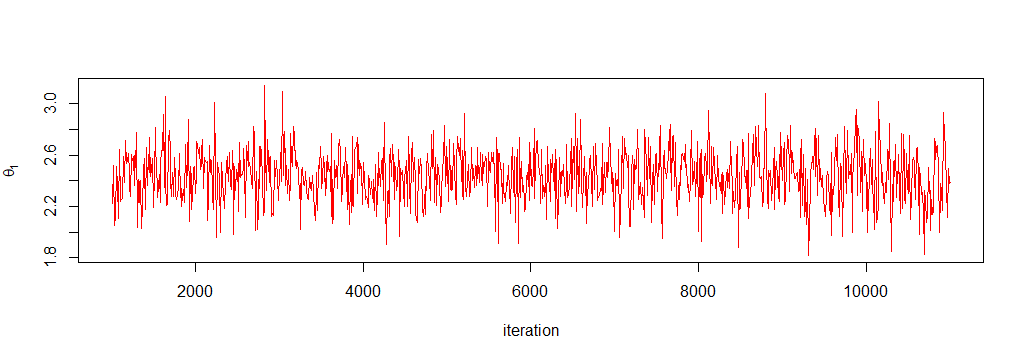
\includegraphics[width = \textwidth]{theta1_convergence.png}
    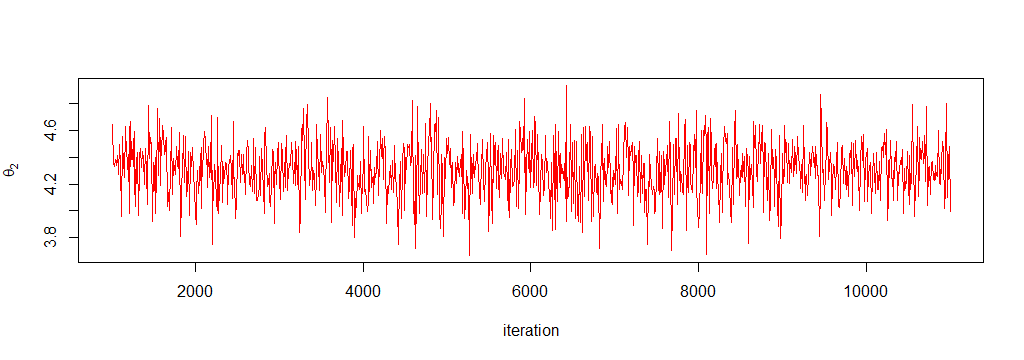
\includegraphics[width = \textwidth]{theta2_convergence.png}
    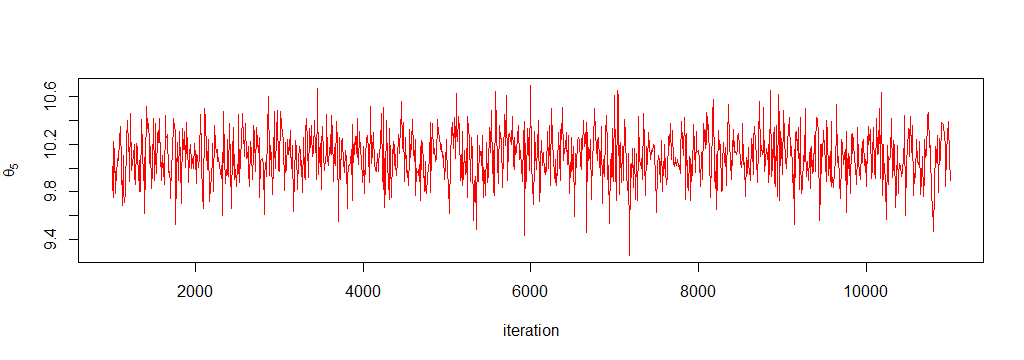
\includegraphics[width = \textwidth]{theta5_convergence.png}
\end{figure}


The estimates obtained from Gibbs sampling using WinBUGS software are given in the following table.

\begin{table}[h]
    \centering
    \resizebox*{\textwidth}{!}{
    \begin{tabular}{c|c}
        \toprule
        $(a_1, a_2, b_1, b_2, \mu_0, \sigma_0^2)$ & Posterior mean of $(\theta_1, \dots, \theta_{10})$\\
        \midrule 
        $(10^2, 10^2, 10^2, 10^2, 0, 10^2)$ & (2.345, 4.225, 6.254, 8.106, 10.043, 12.235, 13.947, 15.831, 17.201, 20.054)\\
        $(10^3, 10^2, 10^3, 10^2, 0, 10^3)$ & (2.221, 4.126, 6.188, 8.061, 10.049, 12.247, 13.983, 15.89, 17.311, 20.171)\\
        $(10^2, 10^3, 10^2, 10^3, 0, 10^3)$ & (2.684, 4.482, 6.437, 8.223, 10.084, 12.175, 13.835, 15.657, 16.968, 19.71)\\
        $(10^3, 10^3, 10^3, 10^3, 0, 10^3)$ & (2.394, 4.266, 6.285, 8.121, 10.061, 12.224, 13.919, 15.825, 17.177, 19.989)\\
        $(10^3, 10^3, 10^3, 10^3, 10, 10^2)$ & (2.437, 4.306, 6.326, 8.172, 10.098, 12.263, 13.958, 15.843, 17.216, 20.029)\\
        \bottomrule
    \end{tabular}}
    \caption{Estimates of population means based on Gibbs Sampling using WinBUGS}
\end{table}


As expected, the results are quite similar to that obtained using the custom code for Gibbs sampling.


\end{solution*}
\pagebreak


\begin{center}
    \vspace*{5cm}
    \rule{0.8\linewidth}{0.1pt}\\
    \vspace*{2cm}
    \Huge \textbf{Thank You}\\
    \vspace*{2cm}
    \rule{0.8\linewidth}{0.1pt}
    \vfill
\end{center}


\end{document}